%%%%%%%%%%%%%%%%%%%%%%%%%%%%%%%%%%%%%%%%%%%%%%%%%%%%%%%
%                  File: OPTICAmeetings.tex           %
%                  Date: 31 July 2023                 %
%                                                     %
%     For preparing LaTeX manuscripts for submission  %
%     submission to Optica meetings and conferences   %
%                                                     %
%         (c) 2018-2022 Optica Publishing Group       %
%%%%%%%%%%%%%%%%%%%%%%%%%%%%%%%%%%%%%%%%%%%%%%%%%%%%%%%

\documentclass[letterpaper,11pt]{article} 
%% if A4 paper needed, change letterpaper to A4

\usepackage{opticameet3} %% use version 3 for proper copyright statement

%% provide authormark
\newcommand\authormark[1]{\textsuperscript{#1}}

%% standard packages and arguments should be modified as needed
\usepackage{amsmath,amssymb}
\usepackage[hyphens]{url}
\usepackage[breaklinks=true]{hyperref} %pdflatex
\hypersetup{
	breaklinks=true
}
\renewcommand{\arraystretch}{1.3}
%\usepackage[breaklinks,colorlinks=true,bookmarks=false,citecolor=blue,urlcolor=blue]{hyperref} %latex w/dvipdf
\usepackage{array}
\usepackage{amsmath}
\usepackage{tabularx}
\usepackage{geometry}
\newcolumntype{L}[1]{>{\raggedright\arraybackslash}p{#1}} % linksbündig mit fester Breite
\newcolumntype{R}[1]{>{\raggedleft\arraybackslash}p{#1}}  % rechtsbündig mit fester Breite


\begin{document}

\title{Techno-Economic and Environmental Pre-Assessment of Large-Scale Heat Pumps Using the HeatSHIFT Webtool}

% \author{Author name(s)}
% \address{Author affiliation and full address}
% \email{e-mail address}

\author{Verena Jetzinger,\authormark{1,*} Matthias Finkenrath,\authormark{1}, Luca Rieger, \authormark{1} \\ Michael Riegger \authormark{1} and Christian Pressa\authormark{1}}

\vspace{5mm}

\address{\authormark{1}Institute for Energy and Propulsion Technology, University of Applied Sciences Kempten, Bahnhofstraße 61, 87435 Kempten (Allgäu), Germany}


\email{\authormark{*}verena.jetzinger@hs-kempten.de} %% email address is required

%% Do not add a copyright statement. Optica will add it.

\begin{abstract}
	Heat pumps are expected to play a central role in the decarbonization of the heating sector. Despite their technical potential to cover Germany’s entire heat demand up to 200\,\textdegree{}C, the market uptake -- particularly for large-scale applications -- remains slow. Complex planning and approval procedures often hinder early project development.
	
	To address this challenge, the HeatSHIFT project has developed a web-based preliminary design tool that enables the systematic assessment and comparison of large-scale heat pump systems. The tool incorporates technical, economic, and environmental evaluations and requires minimal user input by providing representative default values and simplified equations. It includes refrigerant selection, process simulation, cost estimation, subsidy modeling, and scenario as well as sensitivity analyses.
	
	The tool is intended to support planners, utilities, and municipal stakeholders in making data-driven decisions and accelerating the deployment of large-scale heat pumps.
\end{abstract}



\tableofcontents
\vspace{5mm}


\noindent
\framebox{%
	\begin{minipage}{\textwidth}
		\vspace{1em}
		
		\textbf{$\:$ Abbreviations}
		
		\vspace{1em}
		
		\begin{tabularx}{\textwidth}{@{} R{2cm} X R{2cm} X @{}}
			CHP & Combined heat and power &
			DH & District heating \\[0.25em]
			
			COP & Coefficient of performance &
			KWKG & Combined Heat and Power Act \\[0.5em]
			
			NPV & Net present value &
			BAFA & Federal Office for Economic Affairs and Export Control \\[0.5em]
			
			BEW & Federal Funding for Efficient Heating Networks &
			SCOP & Seasonal coefficient of performance \\[0.5em]
			
			GWP & Global Warming Potential &
			ODP & Ozone Depletion Potential \\[0.5em]
			
		\end{tabularx}
			
		\vspace{1em}
		
		\textbf{$\:$ Nomenclature}
		
		\vspace{1em}
		
		\begin{tabularx}{\textwidth}{@{} R{2cm} X R{2cm} X @{}}
			$\dot{Q}$ & Thermal load (kW) &
			$P$ & Power (kW) \\[0.5em]
			
			$T$ & Temperature (K) &
			$\eta_g$ & Second law efficiency \\[0.5em]
						
		\end{tabularx}
	\end{minipage}%
}

\vspace{2em}

\section{Introduction}

Heat pumps are considered a key technology for the energy transition. According to \cite{agorarollout}, heat pumps are technically capable of meeting the entire heat demand in Germany up to temperatures of 200\,\textdegree{}C. This demand currently accounts for over 75\% of the national natural gas consumption. As such, heat pumps represent a central pillar in the decarbonization of the heating sector. However, \cite{agorarollout} also highlights that the market ramp-up -- especially for large-scale heat pumps -- remains slow. This is primarily due to complex planning and permitting procedures.

As part of the research project \textit{HeatSHIFT}, a preliminary design tool has been developed to support the early-stage assessment and comparison of large-scale heat pump systems. In the following sections, the HeatSHIFT project is briefly introduced, and the structure, functionality, and application of the tool are presented in detail.




\section{HeatSHIFT research project}

In order to achieve the German governments climate targets for 2045 and the associated extensive decarbonization of heat supply, district heating (DH) plays a key role. Against the backdrop of emission reduction and the simultaneous enhancement of supply security, the research project HeatSHIFT aims to investigate efficient integration options for high-temperature heat pumps in DH networks. The analyses focus on existing DH systems with high supply temperatures of 120 $^\circ$C and above.

The core objective of the project is the systematic investigation and both technical and economic evaluation of the use of high-temperature heat pumps through process simulation, taking into account various heat sources and high-temperature heat pump technologies. To this end, realistic process simulation models of high-temperature heat pumps and combined heat and power (CHP) plants -- particularly biomass and waste-to-energy plants -- are developed and combined based on data provided by the project partners. On the basis of validated process simulation models, the integration of high-temperature heat pumps is optimized, and an economic evaluation is performed. 

Furthermore, a simplified tool for the preliminary design of heat pump applications is developed for heat suppliers. This tool is introduced and described in more detail in the following section.

\begin{figure}[!ht] 
	\centering 
	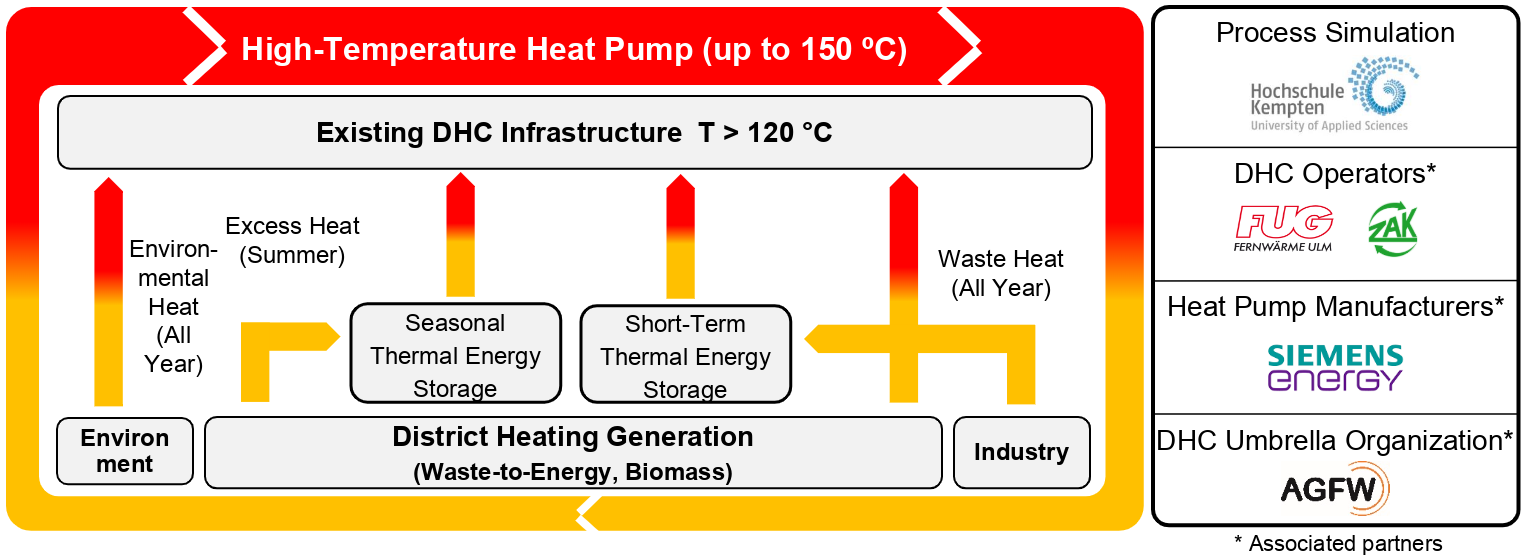
\includegraphics[width=\linewidth]{Abbildungen/heatshift.png} 
	\label{fig:heatshift} 
\end{figure}


\section{Webtool}

	The tool aims at facilitating the initial steps in the planning process of large-scale heat pump systems, enabling a systematic comparison of available options, and supporting data-driven decision-making. It is intended for planners, utility companies, research institutions, and municipal decision-makers who seek to actively contribute to the transition toward a climate-neutral heat supply.
	
	It is designed to operate with minimal prior information. To enable its application even in the absence of detailed input data, representative default values and approximate equations have been predefined for all key parameters. These values are derived from current literature, standard assumptions, and official sources. While they provide a useful basis for initial orientation, they should be adjusted accordingly whenever more accurate information becomes available.
	
	The webtool is structured into three main components: technical, economic, and environmental assessment. These components, along with a preceding disclaimer, are presented in the following subsections.

	\subsection{Disclaimer}
	
	The authors explicitly disclaim any liability for the accuracy, completeness, or applicability of the results generated by this tool. The methodological framework and default values are intended to support preliminary assessments of the technical, economic and environmental performance of large-scale heat pump systems. The results are not designed to replace professional engineering judgment or detailed project-specific planning. Users are therefore advised to validate the results with site-specific data and consult relevant experts before drawing any conclusions or making investment decisions.
	
	\subsection{Technological evaluation}
	
	To assess the technical feasibility of integrating a heat pump into a heating system, the tool first determines suitable refrigerants based on the specified temperature levels. Subsequently, a heat pump is simulated using the refrigerant selected by the user. Key performance indicators and process variables are provided as outputs. The only required inputs are the inlet and outlet temperatures of the heat source and heat sink, as well as either the required useful heat output or the available thermal power from the heat source. The user may choose which of the two thermal power parameters to specify.

		\subsubsection{Refrigerant selection}
		
		The tool considers the following refrigerants: R32, R1270, R290, R717, R1234yf, R134a, R227ea, R600a, R236fa, R600, R718, R245fa, R1233zd(E), R245ca, and R601. To define the applicable temperature range for each refrigerant, the lower temperature boundary is set to 5 K above the boiling temperature at a pressure of 1 bar. For R718, an exception is made due to its thermophysical properties, and a reference pressure of 611.655 Pa is applied. The upper temperature boundary is defined as 15 K below the respective critical temperature \cite{vdi4646}. Thermophysical property data are retrieved from the \textit{CoolProp} database \cite{coolprop}. The resulting temperature ranges are summarized in Table~\ref{tab:kaeltemittel}.
		
		\begin{table}[!ht] 
			\centering 
			\caption{Applicable temperature ranges for selected refrigerants}
			 \begin{tabular}{ l c c } 
			 	\hline 
			 	\textbf{Refrigerant} & \textbf{Lower temperature limit [$^{\circ}$C]} & 
			 	\textbf{Upper temperature limit [$^{\circ}$C]} \\ 
			 	\hline R32 & $-46{,}91$ & $66{,}11$ \\
			 	 R1270 & $-42{,}91$ & $76{,}06$ \\ 
			 	 R290 & $-37{,}41$ & $81{,}74$ \\ 
			 	 R717 & $-28{,}58$ & $117{,}41$ \\ 
			 	 R1234yf & $-24{,}78$ & $79{,}70$ \\ R134a & $-21{,}36$ & $86{,}06$ \\ 
			 	 R227ea & $-11{,}65$ & $86{,}75$ \\ 
			 	 R600a & $-7{,}08$ & $119{,}67$ \\ 
			 	 R236fa & $3{,}20$ & $109{,}92$ \\ 
			 	 R600 & $4{,}16$ & $136{,}98$ \\ 
			 	 R718 & $5{,}01$ & $358{,}95$  \\ 
			 	 R245fa & $19{,}72$ & $138{,}86$ \\ 
			 	 R1233zd(E) & $22{,}91$ & $151{,}45$ \\ 
			 	 R245ca & $29{,}92$ & $159{,}42$ \\ 
			 	 R601 & $40{,}67$ & $181{,}55$ \\ 
			 	 \hline \end{tabular} 
			 \label{tab:kaeltemittel} 
		\end{table}
		
		From the set of refrigerants suitable for the specified operating temperature range, the user selects one for subsequent process simulation, as illustrated in Figure~\ref{fig:auswahl_km}.
		
		\begin{figure}[!ht] 
			\centering 
			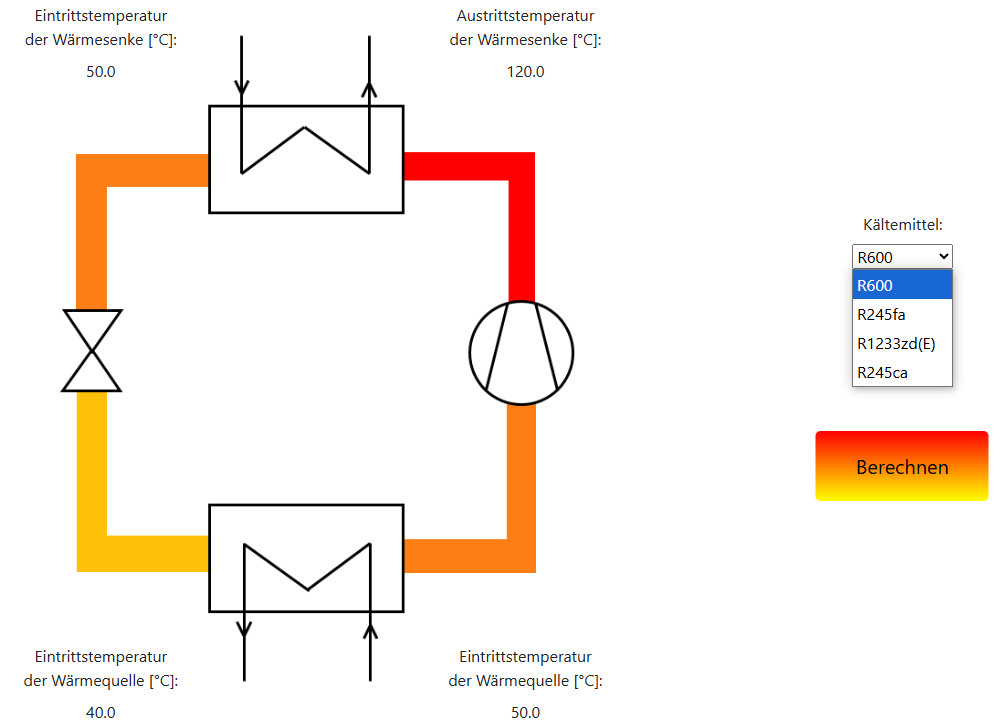
\includegraphics[width=0.8\textwidth]{Abbildungen/Auswahl_KM.png} 
			\caption{Example selection of refrigerants matching the operating temperature range} \label{fig:auswahl_km} 
			\end{figure}
		
		\subsubsection{Cycle simulation}
		
		Based on the selected refrigerant, the thermodynamic cycle of a single-stage vapor-compression heat pump is subsequently simulated. A terminal temperature difference of 5 K is assumed for both heat exchangers, and a superheat of 5 K is specified at the compressor outlet. The isentropic compressor efficiency is assumed to be 85 \%, while the mechanical efficiency is set to 95 \%.
		
		Depending on the user input -- either the useful heat output $\dot{Q}{sink}$ or the heat input from the source $\dot{Q}{source}$ -- the respective counterpart, as well as the compressor’s electrical power consumption $P_{el}$, is determined using thermophysical property data from CoolProp. The coefficient of performance (COP) of the heat pump is subsequently calculated according to Equation~\ref{eq:cop}.
		
		\begin{equation}
			\text{COP} = \frac{\dot{Q}_{sink}}{P_{el}}
			\label{eq:cop}
		\end{equation}
		
		Furthermore, the theoretical Carnot COP and the second law efficiency $\eta_{g}$ of the heat pump are computed using Equations~\ref{eq:cop_carnot} and~\ref{eq:guetegrad}, respectively. These metrics serve to evaluate the thermodynamic quality of the process. For the calculation of the Carnot COP, the boiling temperatures $T_{boil,up}$ and $T_{boil,low}$ corresponding to the respective pressure levels are applied.
		
		\begin{equation}
			\text{COP}_{\text{Carnot}} = \frac{T_{boil,up}}{T_{boil,up} - T_{boil,low}}
			\label{eq:cop_carnot}
		\end{equation}
		
		\begin{equation} \eta_{g} = \frac{\text{COP}}{\text{COP}_{\text{Carnot}}} \label{eq:guetegrad} \end{equation}
		
		In addition, the mass flow rates of water on both the source and sink sides are determined to quantify the thermal exchange at the respective temperature levels. Finally, the process is visualized in a $p$-$h$ diagram, as shown in Figure~\ref{fig:ph-diagram}.
		
		\begin{figure}[!ht] 
			\centering 
			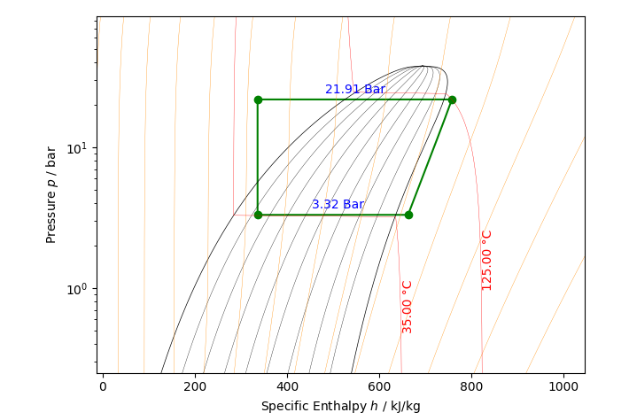
\includegraphics[width=0.8\textwidth]{Abbildungen/ph-diagram.png} 
			\caption{Visualization of a representative process in a $p$-$h$ diagram} 
			\label{fig:ph-diagram} \end{figure}

	\subsection{Economic evaluation}
	
	The economic evaluation requires a range of input parameters. In addition to the investment and operating costs of the heat pump system, system- and operation-specific parameters must be provided, such as the nominal capacity, COP, annual full-load hours, type of heat source, and expected service life. If investment and operating costs are not available, they are estimated based on \cite{pieper2018} and \cite{BAFA2024Modul4}.
	
	Furthermore, economic indicators such as the interest rate, inflation rate, and energy price fluctuations are also of relevance. The electricity price for the purchased electricity must be specified. It can also be indicated whether industrial electricity tariffs apply. Default values are based on \cite{statisitischesbundesamt2024}. Any share of electricity from self-generation is not included in the electricity cost calculation.
	
	The economic benefit is defined as the avoided cost of natural gas. Therefore, the gas price must also be provided. The default value is likewise taken from \cite{statisitischesbundesamt2024}.
	
	Finally, it can be specified whether the heat pump is to be integrated into a CHP system. If so, financial support under the Combined Heat and Power Act (KWKG) may be available. In this case, the electrical and thermal output of the CHP system must also be specified.
	
	The economic evaluation comprises not only the calculation of levelized cost of heat but also includes a scenario and sensitivity analysis as well as an option to estimate potential subsidies.
	
		\subsubsection{Scenario analysis}
		
		The scenario analysis is conducted in accordance with DIN 17463. The standard recommends a parameter variation of 50\%, unless other values are known \cite{vdi17463}. The parameters subjected to variation include the annual useful energy, the investment lifetime, investment costs, discount rate, operating costs excluding energy costs, electricity costs, avoided gas costs, share of self-generated electricity, inflation, and energy price volatility. 
		
		The resulting key figures are the net present value (NPV) and the payback period. The development of the NPV is also illustrated graphically as examplarily shown in Figure \ref{fig:scenario-analysis} as well as in tabular form.
		
		\begin{figure}[!ht] 
			\centering 
			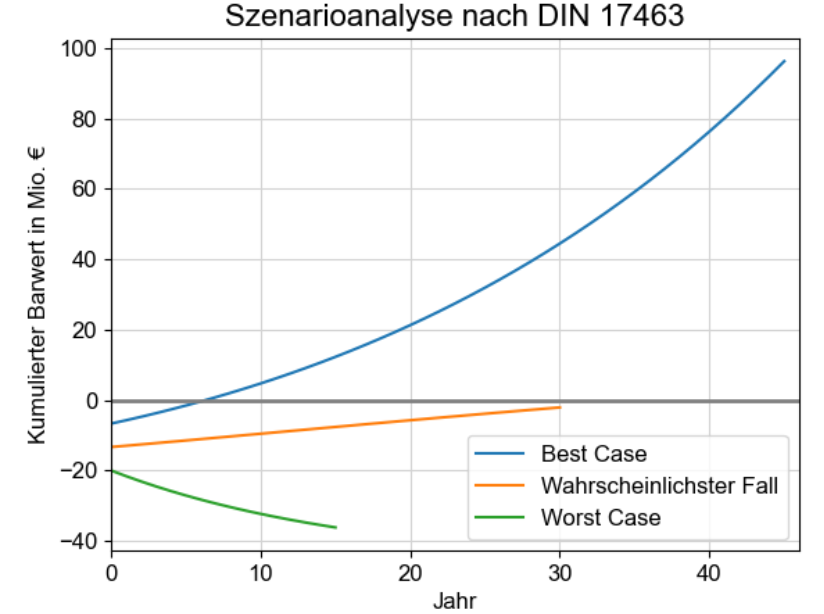
\includegraphics[width=0.8\linewidth]{Abbildungen/scenario-analysis.png}
			\caption{Scenario analysis according to DIN 17463} 
			\label{fig:scenario-analysis} 
		\end{figure}

		
		\subsubsection{Sensitivity analysis}
		
		The sensitivity analysis is likewise conducted in accordance with DIN 17463. For this purpose, the parameters annual useful energy, investment lifetime, investment costs, discount rate, operating costs excluding energy costs, electricity costs, gas costs, inflation, and energy price volatility are each varied by 50\%. The impact on the NPV is then evaluated. The results are presented both graphically as exemplarily shown in Figure \ref{fig:sensitivity-analysis} and in tabular form.
		
		\begin{figure}[!ht] 
			\centering 
			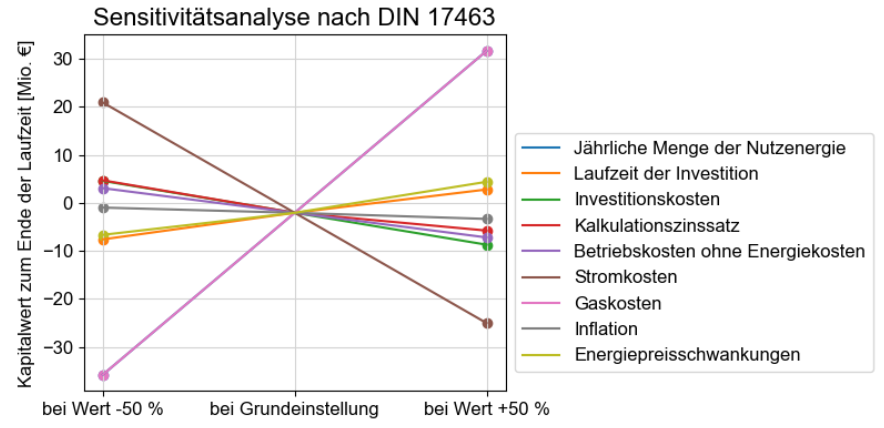
\includegraphics[width=\linewidth]{Abbildungen/sensitivity-analysis.png}
			\caption{Sensitivity analysis according to DIN 17463} 
			\label{fig:sensitivity-analysis} 
		\end{figure}
		
		\subsubsection{Estimation of potential subsidies}
		
		The economic viability of plant operation can be significantly improved through the use of available subsidies. Two potential funding mechanisms are considered in this context. Firstly, a subsidy from the Federal Office for Economic Affairs and Export Control (BAFA) under the Federal Funding for Efficient Heating Networks (BEW funding) may be applicable \cite{BAFA2024}. Additionally, if the heat pump is part of an innovative CHP system, surcharge payments for the generated CHP electricity can be applied for under the KWKG \cite{BAFAKWK}.
		
		The BEW funding options comprise four modules. For heat pump funding, Modules 2 or 3 and Module 4 are relevant. Modules 2 or 3 cover the heat pump as an individual measure and support associated investment costs, while Module 4 serves to subsidize operating costs. Funding under Modules 2 or 3 covers 40\% of the expenses that can be clearly attributed to the individual measure and is capped at the economic viability gap or €100,000,000 \cite{BAFA2024}. The economic viability gap is defined as the NPV over 30 years of operation, assuming an inflation rate of 2\% and a discount rate of 6\% \cite{BAFA2024Modul4}. The funding level under Module 4 depends on the type of electricity generation. Maximum subsidy rates vary depending on whether the electricity is drawn from the grid or generated from a renewable energy source. In the case of mixed electricity sourcing, the subsidy amounts are calculated proportionally. The operating cost subsidy is limited to 90\% of electricity costs. An application may be submitted for a maximum of €100,000,000 or the economic viability gap. A minimum efficiency of the system must be demonstrated through a seasonal coefficient of performance (SCOP) of at least 2.5. The funding is granted for a period of 10 years and is disbursed annually \cite{BAFA2024}.
		
		To obtain funding for the use of a heat pump within the framework of an innovative CHP system under the KWKG, several requirements must be fulfilled. The entire system must consist of a CHP plant with an electrical output of more than 10~MW, combined with a heat pump and an additional electric heat generator operated under a joint control system. These heat generators must feed into a common heat network. Furthermore, the heat pump must be powered by electricity or a gaseous medium and must achieve an annual performance factor of at least 1.25 \cite{BAFAKWK}. The specific requirements are highly complex and must be examined in detail on a case-by-case basis, including the level of surcharge payments. The surcharge is granted as an additional funding component for the generated CHP electricity. The eligible subsidy amount is determined based on the share of innovative heat relative to the reference heat. The reference heat is defined as the useful heat of the CHP system at 3,000 full load hours per year combined with the useful heat of the heat pump \cite{BAFAKWK}. Table~\ref{tab:kwkgzuschlag} shows the surcharge in accordance with KWKG~§~7a.
		
		
		\begin{table}[!ht] 
			\centering 
			\caption{Surcharges pursuant to KWKG § 7a for innovative renewable heat}
			\begin{tabular}{ c c } 
				\hline 
				\textbf{Share of innovative renewable heat [\%]} & \textbf{Surcharge [ct/kWh CHP electricity]}  \\ 
				\hline 
				$\geq$ 5 \% & 0.4 \\
				$\geq$ 10 \% & 0.8 \\
				$\geq$ 15 \% & 1.2 \\
				$\geq$ 20 \% & 1.8 \\
				$\geq$ 25 \% & 2.3 \\
				$\geq$ 30 \% & 3.0 \\
				$\geq$ 35 \% & 3.8 \\
				$\geq$ 40 \% & 4.7 \\
				$\geq$ 45 \% & 5.7 \\
				$\geq$ 50 \% & 7.0 \\
				\hline 
			\end{tabular} 
			\label{tab:kwkgzuschlag} 
		\end{table}
		
		

	
	\subsection{Ecological evaluation}
	
	To provide an initial estimate of the environmental impact of the potential heat pump system, various indicators are determined under the section for ecological assessment. In addition to the nominal capacity and COP of the heat pump, the user must specify the annual full-load hours, service life, and selected refrigerant. Moreover, the electricity generation source used to operate the heat pump must also be selected.
	
	The calculation determines the amount of CO$_2$ emissions that can be avoided annually and over the entire lifetime of the system through the deployment of a large-scale heat pump. For comparison, a reference scenario is considered in which the same amount of useful heat is provided by a natural gas-fired boiler with an assumed boiler efficiency of 95~\%. The emission factor and calorific value of natural gas are taken from \cite{Juhrich2022}, while the emission factors for various electricity generation technologies are based on \cite{Lauf2022} and \cite{Icha2023}. % The comparison is illustrated in Figure~\ref{fig:eingespartes_co2}. 
	
	In addition, information on the selected refrigerant -- such as its safety classification, atmospheric lifetime, Global Warming Potential (GWP), and Ozone Depletion Potential (ODP) \cite{vdi4646} -- is provided to facilitate a more comprehensive understanding of the refrigerant-related environmental impact.
	
%	\begin{figure}[!ht] 
%		\centering 
%		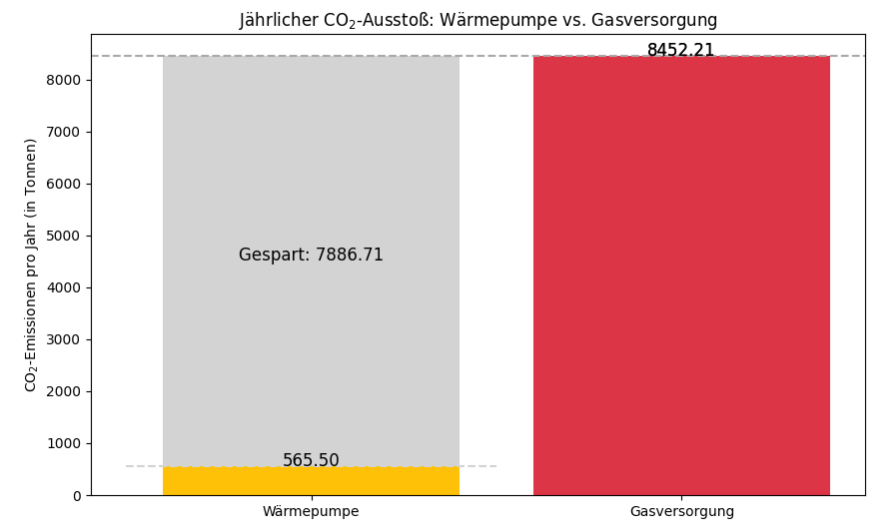
\includegraphics[width=0.8\textwidth]{Abbildungen/Eingespartes-CO2.png} 
%		\caption{Comparison of CO$_2$ emissions avoided using a heat pump system versus a natural gas boiler system} 
%		\label{fig:eingespartes_co2} 
%	\end{figure}

\section{Conclusion}

Large-scale heat pumps represent a promising technology for the decarbonization of the heating sector, particularly within existing DH systems. However, their deployment remains limited due to complex planning processes and a lack of early-stage planning tools. 

The HeatSHIFT webtool addresses this gap by providing a freely accessible, user-friendly platform for the preliminary techno-economic and environmental evaluation of large-scale heat pump systems. It supports informed decision-making by combining refrigerant selection, cycle simulation, cost estimation, scenario and sensitivity analysis, and ecological assessment within a single framework.

By relying on validated default values and simplified modeling approaches, the tool enables a structured comparison of technology options, even in the absence of detailed input data. It thus provides valuable orientation for planners, utilities, and policymakers committed to accelerating the heat transition.


\vspace{5mm}

\begin{thebibliography}{99} %% use BibTeX or add references manually
	
\bibitem{agorarollout} Agora Energiewende, Fraunhofer IEG (2023). \textit{Roll-out von Großwärmepumpen in Deutschland. Strategien für den Markthochlauf in Wärmenetzen und Industrie}.

\bibitem{vdi4646} VDI 4646 - Entwurf (2024). \textit{Anwendung von Großwärmepumpen}.

\bibitem{coolprop} Bell, Ian et al. (2024). \textit{CoolProp: An open-source reference-quality thermophysical property library}. Industrial \& Engineering Chemistry Research, 53(6), 2498-2508. \\
\url{https://doi.org/10.1021/ie403786m}

\bibitem{pieper2018} Pieper, Henrik et al. (2018). \textit{Allocation of investment cost for large-scale heat pumps supplying district heating}. Energy Procedia. \\
\url{https://doi.org/10.1016/j.egypro.2018.07.104}.

\bibitem{BAFA2024Modul4} Bundesamt für Wirtschaft und Ausfuhrkontrolle (2024). \textit{Bundesförderung für effiziente Wärmenetze (BEW) - Modul 4: Berechnungstool Wirtschaftlichkeitslückenberechnung - Wärmepumpe (XLSX)}. \\
\url{https://www.bafa.de/DE/Energie/Energieeffizienz/Waermenetze/Effiziente_Waermenetze/effiziente_waermenetze_node.html}

\bibitem{statisitischesbundesamt2024} Statistisches Bundesamt (Destatis) (2024). \textit{Erdgas- und Stromdurchschnittspreise}. \\
\url{https://www.destatis.de/DE/Themen/Wirtschaft/Preise/Erdgas-Strom-DurchschnittsPreise/_inhalt.html} (Stand: 27.03.2024)

\bibitem{vdi17463} DIN EN 17463 (2021). \textit{Bewertung von energiebezogenen Investitionen (VALERI)}.

\bibitem{BAFA2024} Bundesamt für Wirtschaft und Ausfuhrkontrolle (2024). \textit{Bundesförderung für effiziente Wärmenetze (BEW)}. \\
\url{https://www.bafa.de/DE/Energie/Energieeffizienz/Waermenetze/Effiziente_Waermenetze/effiziente_waermenetze_node.html}

\bibitem{BAFAKWK} Bundesamt für Wirtschaft und Ausfuhrkontrolle (2018). \textit{Merkblatt für innovative KWK-Systeme}.

\bibitem{Juhrich2022} Juhrich, Kristina (2022). \textit{CO$2$-Emissionsfaktoren für fossile Brennstoffe}. Reihe Climate Change \textbar\ 28/2022. Umweltbundesamt, Juni 2022. \\
\url{https://www.umweltbundesamt.de/publikationen/co2-emissionsfaktoren-fuer-fossile-brennstoffe-0}

\bibitem{Lauf2022} Lauf, Thomas et al. (2022). \textit{Emissionsbilanz erneuerbarer Energieträger 2021 - Bestimmung der vermiedenen Emissionen im Jahr 2021}. Reihe Climate Change \textbar\ 50/2022. Umweltbundesamt, Dezember 2022. \\
\url{https://www.umweltbundesamt.de/publikationen/entwicklung-der-spezifischen-treibhausgas-9}

\bibitem{Icha2023} Icha, Petra et al. (2023). \textit{Entwicklung der spezifischen Treibhausgas-Emissionen des deutschen Strommix in den Jahren 1990 - 2022}. Reihe Climate Change \textbar\ 20/2023. Umweltbundesamt, Mai 2023. \\
\url{https://www.umweltbundesamt.de/publikationen/entwicklung-der-spezifischen-treibhausgas-9}

\bibitem{iso817} ISO 817 (2014). \textit{Refrigerants - Designation and safety classification}



\end{thebibliography}

\end{document}
